% Figure 1 (study design) for "Beyond CTI Reporting" (AICS @ AAAI-27).
% Standalone TikZ; compile with pdflatex to produce fig_method.pdf.
% Canvas is 505 x 164 bp, the same size as the previous fig_method.pdf,
% so 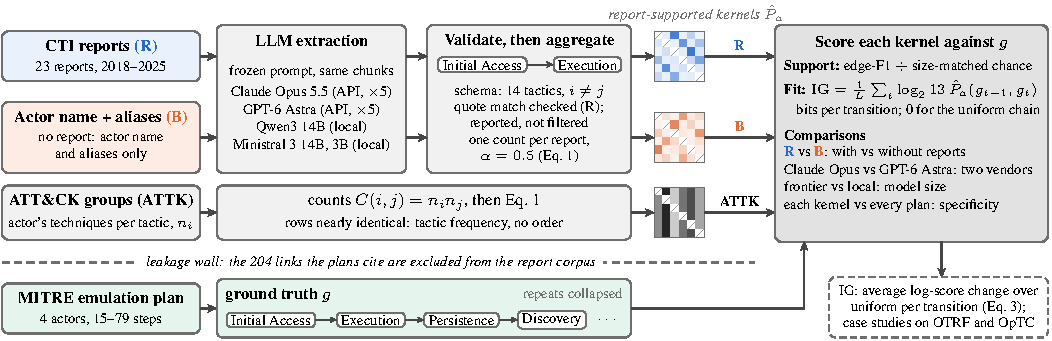
\includegraphics[width=\textwidth]{fig_method} needs no change.
\documentclass[border=0pt]{standalone}
\usepackage{times}
\usepackage{amsmath}
\usepackage{tikz}
\usetikzlibrary{arrows.meta}

\definecolor{Rblue}{RGB}{38,104,206}
\definecolor{Borange}{RGB}{226,104,52}
\definecolor{edge}{RGB}{110,110,110}
\definecolor{ink}{RGB}{70,70,70}
\definecolor{fillR}{RGB}{233,241,252}
\definecolor{fillB}{RGB}{252,236,228}
\definecolor{fillA}{RGB}{241,241,241}
\definecolor{fillP}{RGB}{229,244,237}
\definecolor{fillS}{RGB}{226,226,226}
\definecolor{note}{RGB}{110,110,110}

\newcommand{\ttl}{\fontsize{8}{9.4}\selectfont\bfseries}
\newcommand{\bdy}{\fontsize{7}{7.8}\selectfont}
\newcommand{\sub}{\fontsize{7}{7.8}\selectfont\bfseries}

\begin{document}
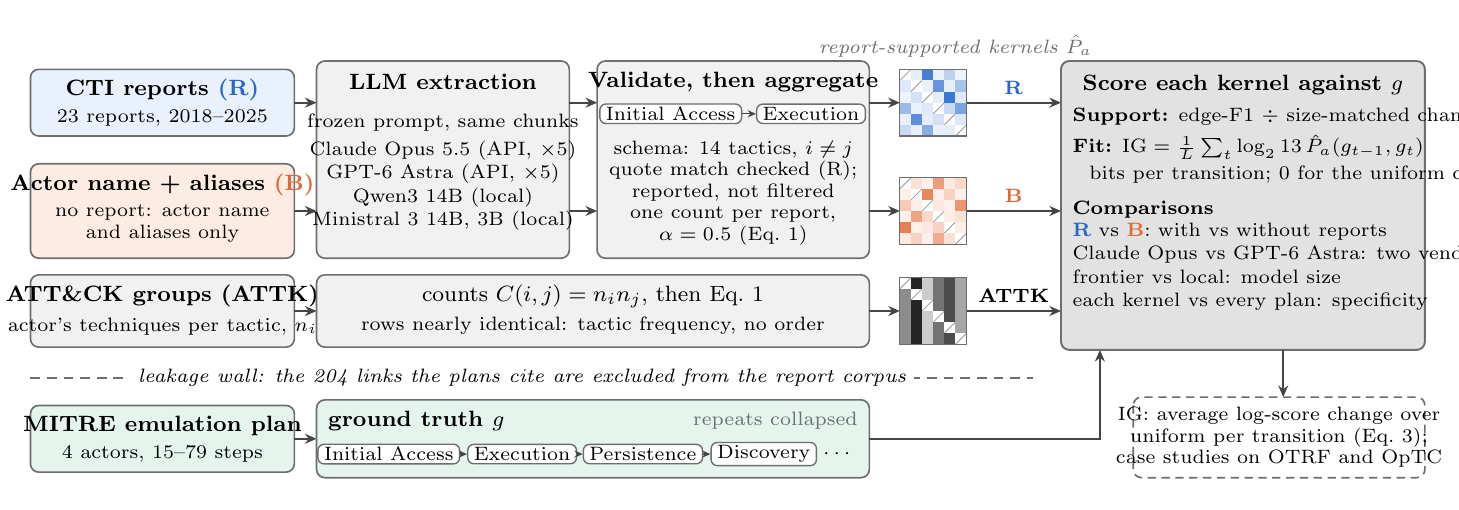
\begin{tikzpicture}[x=1bp,y=-1bp,
  box/.style={draw=edge, line width=0.6pt, rounded corners=3pt},
  arr/.style={-{Stealth[length=4.2pt,width=3.6pt]}, draw=ink, line width=0.7pt},
  chip/.style={draw=edge, line width=0.5pt, rounded corners=2.2pt, fill=white,
               inner xsep=2.2pt, inner ysep=1.1pt, font=\bdy},
  chipar/.style={-{Stealth[length=3pt,width=2.6pt]}, draw=ink, line width=0.5pt},
  txt/.style={inner sep=0pt, align=center},
]
\useasboundingbox (0,0) rectangle (505.08,163.65);

% ---------------- column 1: inputs ----------------
\draw[box, fill=fillR] (1,15) rectangle (96,39);
\node[txt, font={\ttl}] at (48.5,22.5) {CTI reports \textcolor{Rblue}{(R)}};
\node[txt, font={\bdy}] at (48.5,32.5) {23 reports, 2018--2025};

\draw[box, fill=fillB] (1,49) rectangle (96,83);
\node[txt, font={\ttl}] at (48.5,56.5) {Actor name + aliases \textcolor{Borange}{(B)}};
\node[txt, font={\bdy}] at (48.5,70.5) {no report: actor name\\ and aliases only};

\draw[box, fill=fillA] (1,89) rectangle (96,115);
\node[txt, font={\ttl}] at (48.5,96.5) {ATT\&CK groups (ATTK)};
\node[txt, font={\bdy}] at (48.5,107.5) {actor's techniques per tactic, $n_i$};

% ---------------- column 2: LLM extraction ----------------
\draw[box, fill=fillA] (104,12) rectangle (195,83);
\node[txt, font={\ttl}] at (149.5,19.5) {LLM extraction};
\node[txt, font={\bdy}] at (149.5,52) {frozen prompt, same chunks\\[2.4pt]
  Claude Opus 5.5 (API, $\times$5)\\[0.6pt]
  GPT-6 Astra (API, $\times$5)\\[0.6pt]
  Qwen3 14B (local)\\[0.6pt]
  Ministral 3 14B, 3B (local)};

% ---------------- column 3: validate and aggregate ----------------
\draw[box, fill=fillA] (205,12) rectangle (303,83);
\node[txt, font={\ttl}] at (254,19.5) {Validate, then aggregate};
\node[chip] (c1) at (231.5,31) {Initial Access};
\node[chip] (c2) at (282,31) {Execution};
\draw[chipar] (c1.east) -- (c2.west);
\node[txt, font={\bdy}] at (254,59.5) {schema: 14 tactics, $i \neq j$\\
  quote match checked (R);\\
  reported, not filtered\\
  one count per report,\\
  $\alpha = 0.5$ (Eq.~1)};

% ---------------- ATT&CK counts ----------------
\draw[box, fill=fillA] (104,89) rectangle (303,115);
\node[txt, font={\fontsize{8}{9}\selectfont}] at (203.5,96.8) {counts $C(i,j) = n_i n_j$, then Eq.~1};
\node[txt, font={\bdy}] at (203.5,107.3) {rows nearly identical: tactic frequency, no order};

% ---------------- arrows into columns 2 and 3 ----------------
\draw[arr] (96,27) -- (104,27);
\draw[arr] (96,66) -- (104,66);
\draw[arr] (96,102) -- (104,102);
\draw[arr] (195,27) -- (205,27);
\draw[arr] (195,66) -- (205,66);

% ---------------- kernel glyphs (schematic 6x6 matrices) ----------------
\node[txt, font={\fontsize{7.4}{8}\selectfont\itshape}] at (334,6.5) {\textcolor{note}{report-supported kernels $\hat P_a$}};

% #1 = top-left x, #2 = top-left y, #3 = colour, #4 = list of 36 intensities (0-100; -1 = diagonal)
\newcommand{\glyph}[4]{%
  \foreach \v [count=\k from 0] in {#4} {%
    \pgfmathtruncatemacro{\gr}{int(\k/6)}%
    \pgfmathtruncatemacro{\gc}{mod(\k,6)}%
    \ifnum\v<0
      \fill[white] (#1+4*\gc,#2+4*\gr) rectangle ++(4,4);
      \draw[edge!70, line width=0.3pt] (#1+4*\gc,#2+4*\gr+4) -- ++(4,-4);
    \else
      \fill[#3!\v!white] (#1+4*\gc,#2+4*\gr) rectangle ++(4,4);
    \fi
  }%
  \draw[edge, line width=0.4pt] (#1,#2) rectangle ++(24,24);
}
\glyph{314}{15}{Rblue}{-1,12,85,10,30,8, 15,-1,10,70,12,40, 8,20,-1,12,90,15, 45,10,15,-1,25,60, 10,75,12,20,-1,15, 25,10,55,10,12,-1}
\glyph{314}{54}{Borange}{-1,20,10,65,15,25, 10,-1,80,12,30,10, 35,12,-1,15,10,70, 10,60,25,-1,12,20, 85,10,15,30,-1,12, 15,30,10,55,20,-1}
\glyph{314}{90}{black}{-1,85,20,55,70,35, 45,-1,20,55,70,35, 45,85,-1,55,70,35, 45,85,20,-1,70,35, 45,85,20,55,-1,35, 45,85,20,55,70,-1}

% ---------------- arrows into the scoring box ----------------
\draw[arr] (303,27) -- (314,27);
\draw[arr] (303,66) -- (314,66);
\draw[arr] (303,102) -- (314,102);
\draw[arr] (338,27) -- (372,27);
\draw[arr] (338,66) -- (372,66);
\draw[arr] (338,102) -- (372,102);
\node[txt, font={\fontsize{7}{8}\selectfont\bfseries}] at (355,21.5) {\textcolor{Rblue}{R}};
\node[txt, font={\fontsize{7}{8}\selectfont\bfseries}] at (355,60.5) {\textcolor{Borange}{B}};
\node[txt, font={\fontsize{7}{8}\selectfont\bfseries}] at (355,96.5) {ATTK};

% ---------------- scoring box ----------------
\draw[box, fill=fillS, line width=0.7pt] (372,12) rectangle (503,116);
\node[txt, font={\ttl}] at (437.5,20.5) {Score each kernel against $g$};
\node[txt, anchor=west, font={\bdy}] at (376,32) {{\sub Support:} edge-F1 $\div$ size-matched chance};
\node[txt, anchor=west, font={\bdy}] at (376,43) {{\sub Fit:} $\mathrm{IG} = \tfrac{1}{L}\textstyle\sum_t \log_2 13\,\hat P_a(g_{t-1}, g_t)$};
\node[txt, anchor=west, font={\bdy}] at (382,53) {bits per transition; 0 for the uniform chain};
\node[txt, anchor=west, font={\sub}] at (376,65.5) {Comparisons};
\node[txt, anchor=west, align=left, font={\bdy}] at (376,86) {{\bfseries\textcolor{Rblue}{R}} vs {\bfseries\textcolor{Borange}{B}}: with vs without reports\\[0.6pt]
  Claude Opus vs GPT-6 Astra: two vendors\\[0.6pt]
  frontier vs local: model size\\[0.6pt]
  each kernel vs every plan: specificity};

% ---------------- leakage wall ----------------
\draw[edge, line width=0.6pt, dash pattern=on 3.5pt off 2.5pt] (1,126) -- (362,126);
\node[txt, fill=white, inner xsep=3pt, inner ysep=1pt, font={\bdy\itshape}] at (178,126) {leakage wall: the 204 links the plans cite are excluded from the report corpus};

% ---------------- ground truth ----------------
\draw[box, fill=fillP] (1,136) rectangle (96,160);
\node[txt, font={\ttl}] at (48.5,143.5) {MITRE emulation plan};
\node[txt, font={\bdy}] at (48.5,153.5) {4 actors, 15--79 steps};
\draw[arr] (96,148) -- (104,148);

\draw[box, fill=fillP] (104,134) rectangle (303,162);
\node[txt, anchor=west, font={\ttl}] at (108,141.5) {ground truth $g$};
\node[txt, anchor=east, font={\bdy}] at (299,141.5) {\textcolor{note}{repeats collapsed}};
\node[chip] (g1) at (130,153.5) {Initial Access};
\node[chip] (g2) at (178,153.5) {Execution};
\node[chip] (g3) at (221.5,153.5) {Persistence};
\node[chip] (g4) at (265,153.5) {Discovery};
\node[txt, font={\bdy}] (g5) at (292,153.5) {$\cdots$};
\draw[chipar] (g1.east) -- (g2.west);
\draw[chipar] (g2.east) -- (g3.west);
\draw[chipar] (g3.east) -- (g4.west);

\draw[arr] (303,148) -- (386,148) -- (386,116);

% ---------------- IG note ----------------
\draw[arr] (452,116) -- (452,133);
\draw[edge, line width=0.6pt, rounded corners=3pt, dash pattern=on 3pt off 2pt, fill=white] (398,133) rectangle (503,162);
\node[txt, font={\bdy}] at (450.5,147.5) {IG: average log-score change over\\
  uniform per transition (Eq.~3);\\
  case studies on OTRF and OpTC};

\end{tikzpicture}
\end{document}
